\chapter {Protocole Expérimental}

\section{Matériel utilisé}
En ce que concerne les aspects matériels, le robot bimoteur Wifibot v2, équipé d'un ordinateur à bord, sera utilisé comme plateforme mobile. L'acquisition des données est faite par une camera RGB-D Asus Xtion Pro Live. Par rapport au choix logiciel, l'environnement robotique ROS\footnote{Robot Operating System} a été adopté pour avoir les bibliothèques qui permettent de gérer les nuages de points, Freenect, OpenNi2 et PCL\footnote{Point Cloud Library}, et d'autres nombreux outils de contrôle du robot et sauvegarde d'informations.

\section{Setup expérimental}
\label{sec:base_donnees}
Pour évaluer les capacités de reconnaissance du robot, vingt objets de tailles et formes diverses ont été choisis pour être incorporé à la base de connaissance. Ils s'agit d'objets typiques qui peuvent être facilement retrouvés dans un laboratoire ou un bureau. Ensuite, nous avons effectué un tour complet de l'objet avec le robot en sauvegardant les nuage de point et en extrayant les features VFH pour huit positions différentes écartées de 45 degrés à 1.5 mètres de distance. La position correspondent à l'angle zéro a été choisie de manière aléatoire en alignant un des axes de l'objet avec celui du capteur. L'image \ref{fig:setup_expe} des vues d'un objet exemplifie la composition de la base de données. Une liste complète des objets figure en annexe \ref{annexe:dataset}.

\begin{figure}[H]
	\subfloat{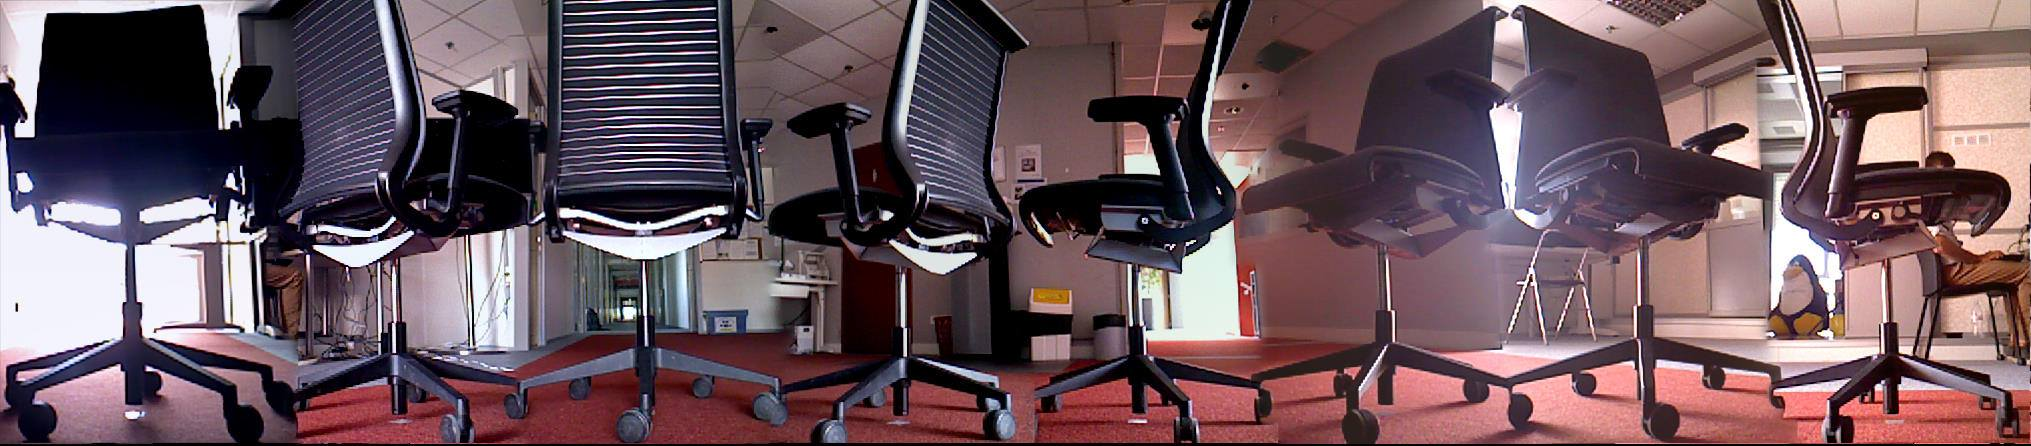
\includegraphics[width=\textwidth]{chair_db.jpg}}		
	\caption{Les huit point de vues de l'objet commençant par la position zéro et en tournant le robot en sens horaire}
	\label{fig:setup_expe}
\end{figure}

\section{Résultats expérimentaux}
\subsection{Comparaison à la reconnaissance mono-vue}
Une première évaluation consiste à faire un tour complet autour de l'objet à reconnaitre pour quatre positions angulaires différentes : $0, 45, 90$ et une dernière choisie de manière aléatoire pour chaque objet. Le robot fait le tour à une vitesse de $0.35 \pm 0.1 m/s$ à une distance de $1.5m$, en enregistrant des images à $1hz$, ansi, une expérience typique est constituée d'environ $25$  images d'angle différent et prendre $25 \pm 3$ seconds. 

La difficulté de l'évaluation vient, premièrement, du fait que la base de donnée a été réalisée avec très peu de vues, ce qui donne lieu à des mauvaise reconnaissance mono-vue lorsque le point de vue observé se situe entre deux vues de la base de connaissance. De plus, la vitesse de déplacement peut générer des images plus floues lors des acquisitions et la modification de l'angle de la caméra\footnote{L'angle entre la base et la tête de la caméra Asus Xtion est facilement modifié.} apportent un obstacle en plus pour le \textit{matching} de descripteurs dans le classificateur K-NN.

Un expérience typique est illustrée dans l'image \ref{fig:resultats_expe} :

\begin{figure}[H]
	\subfloat{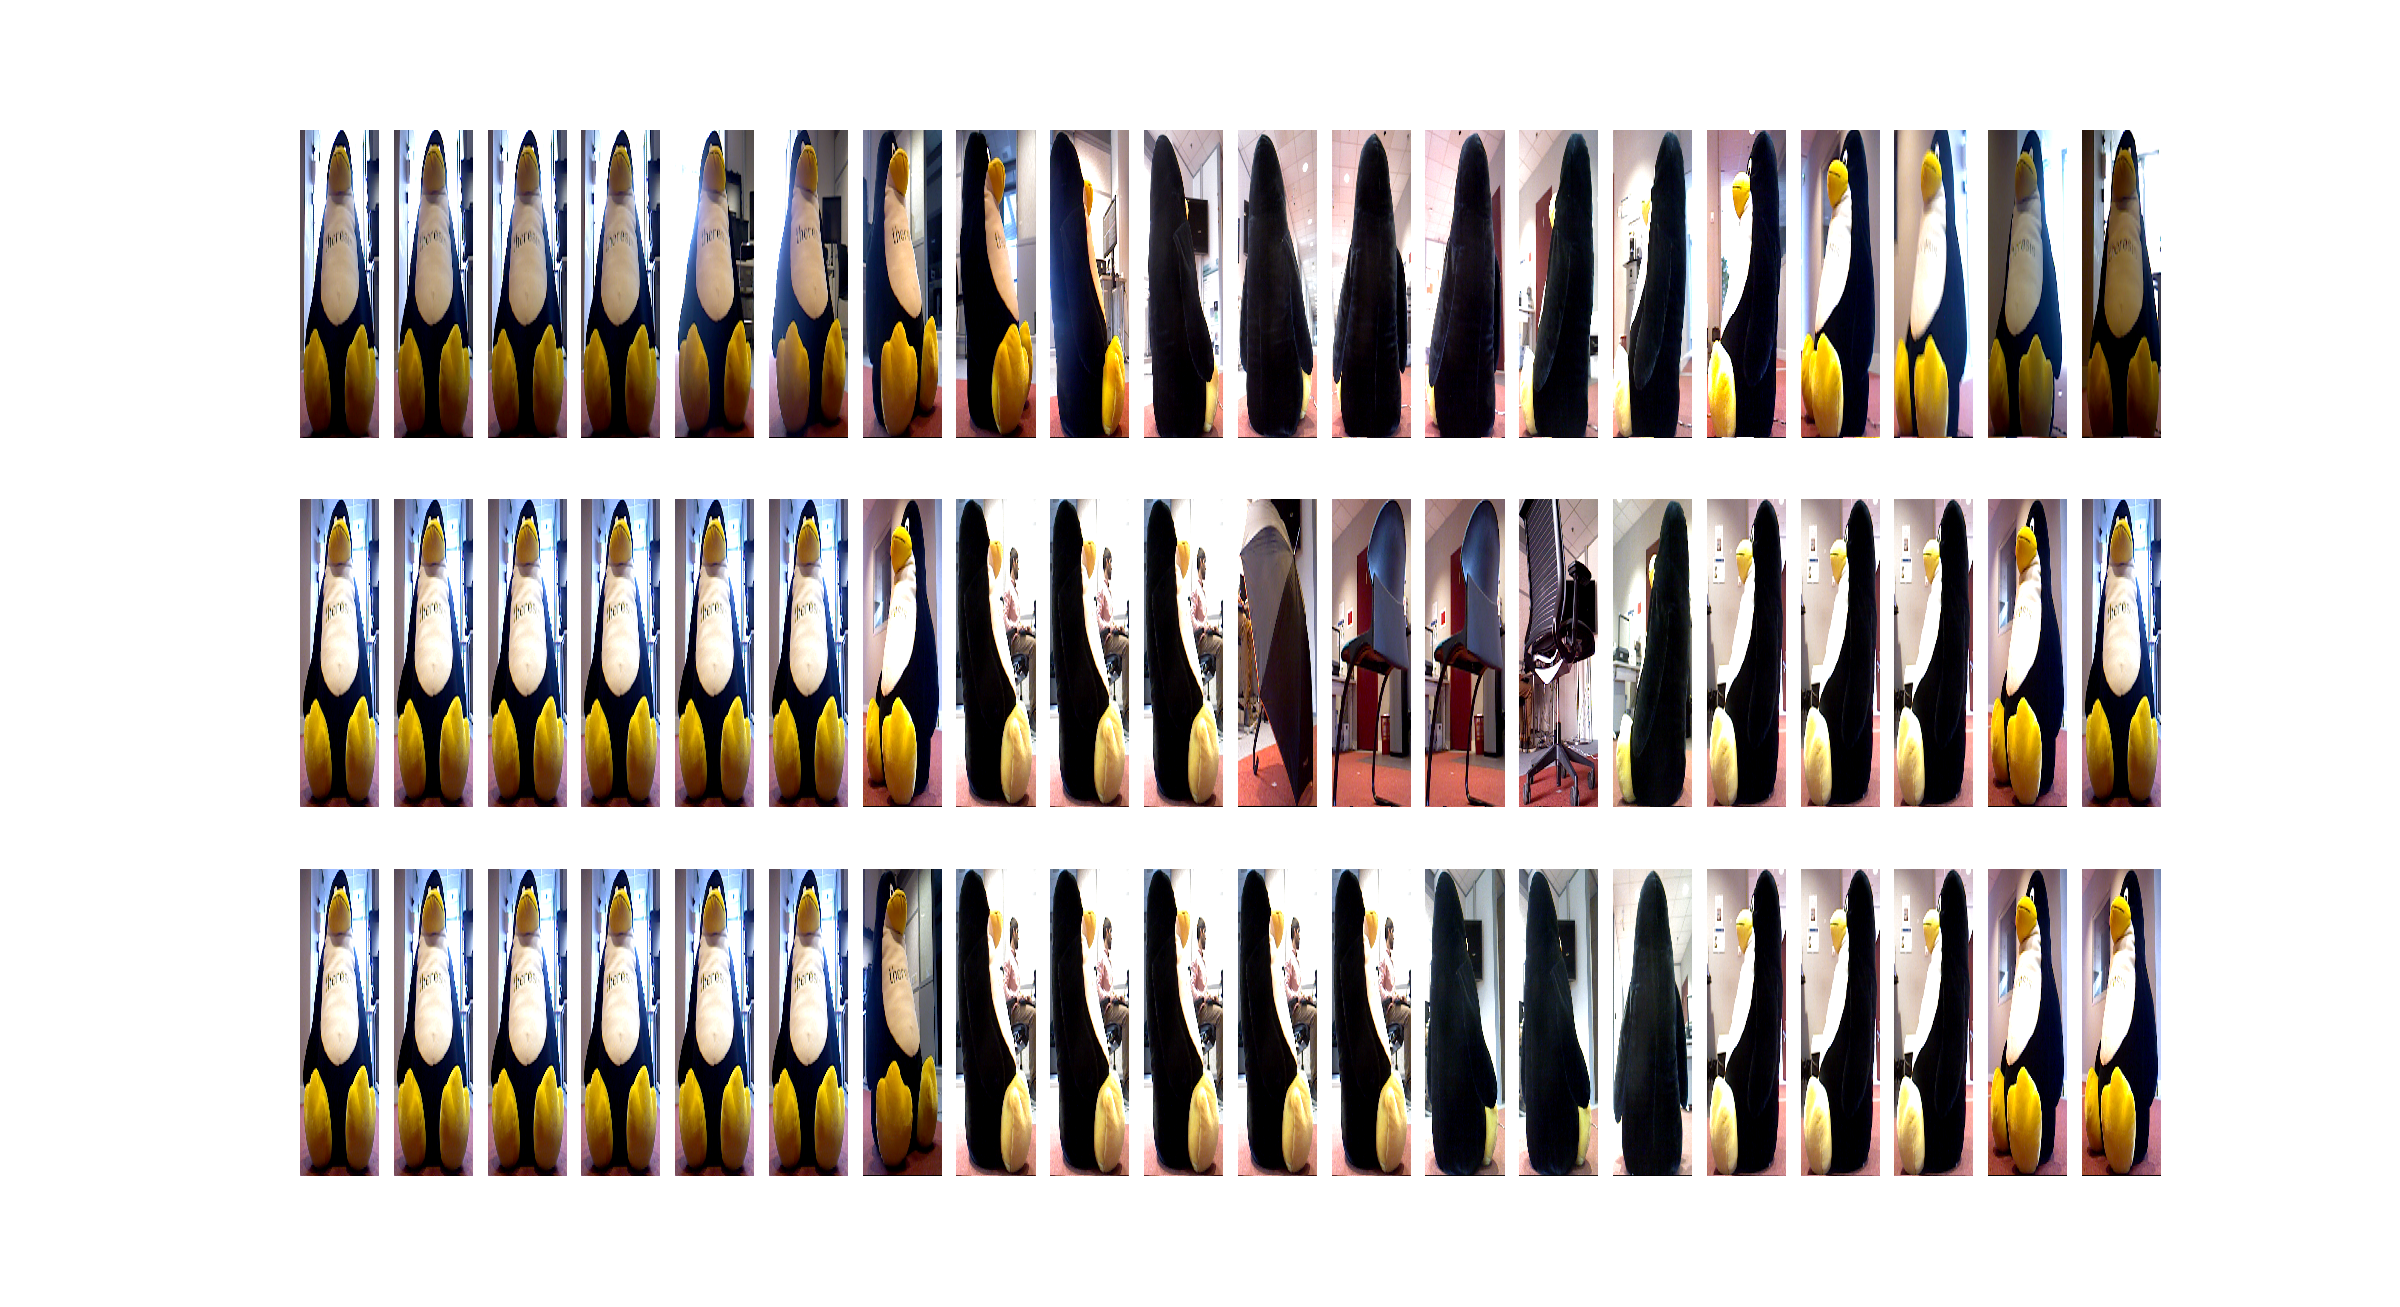
\includegraphics[width=\textwidth]{hmm_example.png}}	
			\caption{\textbf{Expriment typique} - Reconnaissance multi-vue corrige des ambiguïtés et surmonte la mauvaise segmentation lors de la création de la base.}
	\label{fig:resultats_expe}
\end{figure}

La première ligne correspond à la séquence d'images vues par le robot à chaque instant de temps, et donc, l'objet à être reconnu. La seconde ligne, donnée par l'algorithme de reconnaissance, équivaut à la vue la plus probable de l'objet reconnue par le K-plus proches voisins. Il est intéressant remarquer que l'invariance à rotation du descripteur trompe l'estimation de l'orientation en prenant son correspond énantiomorphe dans le premier carré rouge. Autrement, le dos du pinguin étant une grande surface presque plane, il est partiellement retiré par l'étape de segmentation. Ainsi, le nuage de points résultant de ce point de vue n'est pas suffisamment complet pour caractériser correctement l'objet, ce qui induit une mauvaise reconnaissance dans le carré bleu. Au final, on remarque que le traitement apporté par la chaîne de Markov cachée permet de corriger les problèmes d'une base de donnée relativement sparse avec des possibles erreus de segmentation, permettant la correction simultanée de la reconnaissance de l'objet et de son orientation en ligne. 

Le résultat de l'évaluation peut être présenté en forme d'une courbe : nombre de visualisations de l'objet dans les abscisses, par rapport aux taux de reconnaissance d'objet pour chaque système de reconnaissance dans l'estimation de l'objet et de l'orientation.

\begin{figure}[H]
	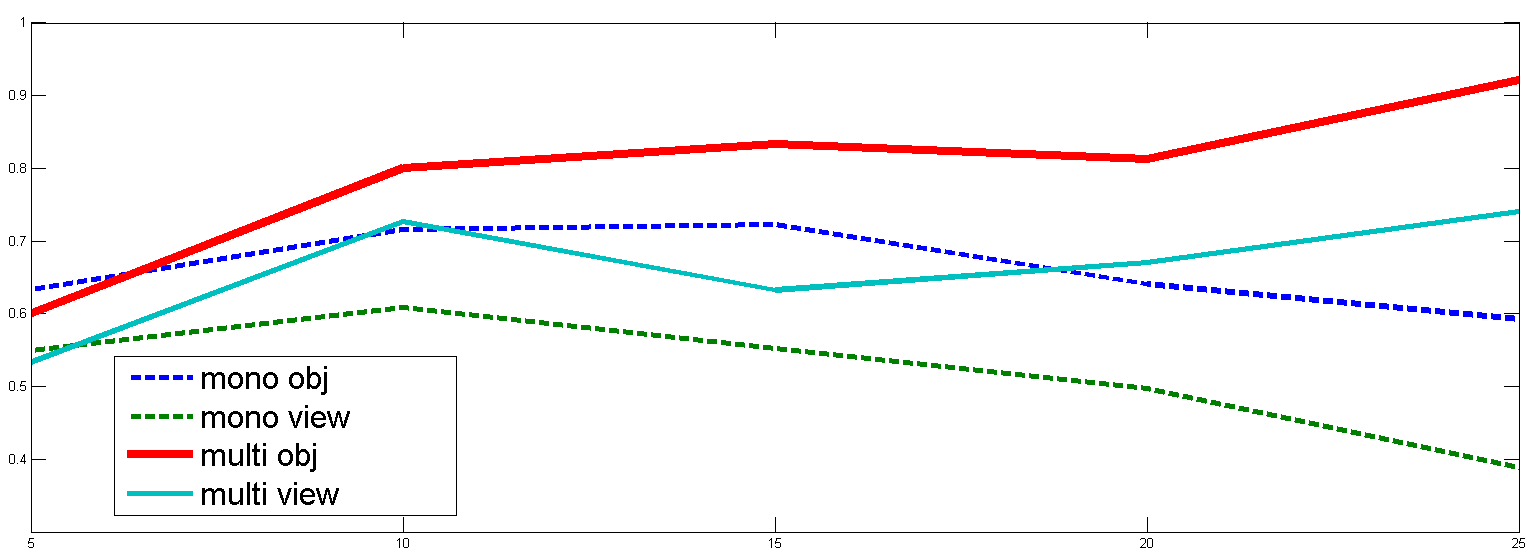
\includegraphics[width=\textwidth]{comp.png}
	\label{fig:comp}
	\caption{\textbf{Résultat de l'évaluation} - Les courbes pointillés représentent le système d'après une seule image fixe (mono-vue), pendent que les complètes correspondent au système multi-vue. Avec un nombre réduit d'images la reconnaissance mono-vue tend à être plus performante . Avec quelques vues différents la taux de reconnaissance commence à monter ayant un écart de 33 \% après le tour complèt avec un valeur absolu de 92\% de réussit pour l'estimation de l'objet et 74 \% pour l'estimation de l'orientation. }		
\end{figure}

La courbe de la figure 3.3 permet conclure, d'abord, que l'algorithme de reconnaissance multi-vue est plus performant que sa correspondent mono-vue lorsque le nombre d'observations augmentes\footnote{Ce fait peut être associé à la démarrage du robot où des images était relativement constants grâce à une vitesse de déplacement moins important au début des séquences.}. Les haut taux de reconnaissance dans En deuxième temps que l'estimation de l'orientation de l'objet est plus difficile que sa reconnaissance, renforcé par le taux inférieur de positifs pour les deux systèmes


%\subsection{Robustesse à l'occlusion}

\subsection{Suivi et reconnaissance multi-cibles}

La deuxième expérimentent correspond à placer des objets présents dans la base de données dans une pièce et conduire le robot en faisant en sorte qu'il les regarde  sous plusieurs points de vues différents. Ce scénario est beaucoup plus complexe que celui d'avant. D'abord les objets occultent uns aux autres, donnant lieux à mauvaises segmentations. Ensuite, le suivi des objets est beaucoup plus complexe où objets proches peuvent être confondus.

La carte finale donnée par l'algorithme est affiché en \ref{fig:multi_map}. Une photo de la pièce aves les objets disposés comme dans l'experiment peut être retrouvé en 3.5. %\ref{fig:exp2}.

\begin{figure}[H]
	\begin{center}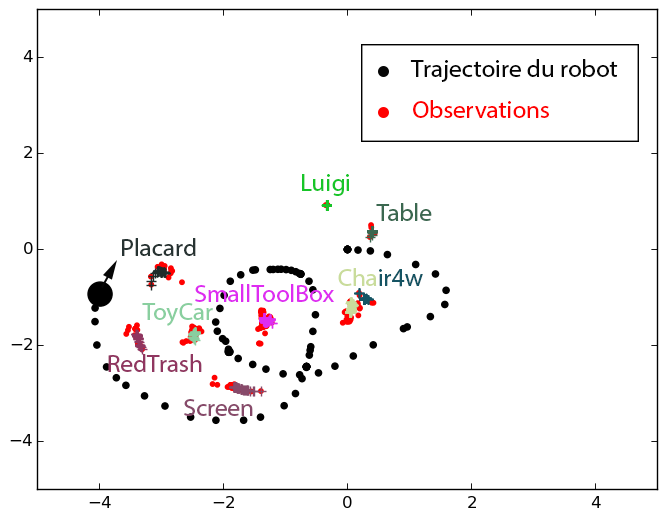
\includegraphics[width=0.8\textwidth]{map.png}\end{center}
	\caption{\textbf{Résultat du déplacement du robot} - Les boules rouges correspodent à les observations des postions des objets, chacun représenté par une croix de couleur différent dans la scène donné par l'algorithme de suivi multi-cibles. En noire la trajectoire du robot bien comme sa dernière position.}	
	\label{fig:multi_map}
\end{figure}

\begin{figure}[H]
	\begin{center}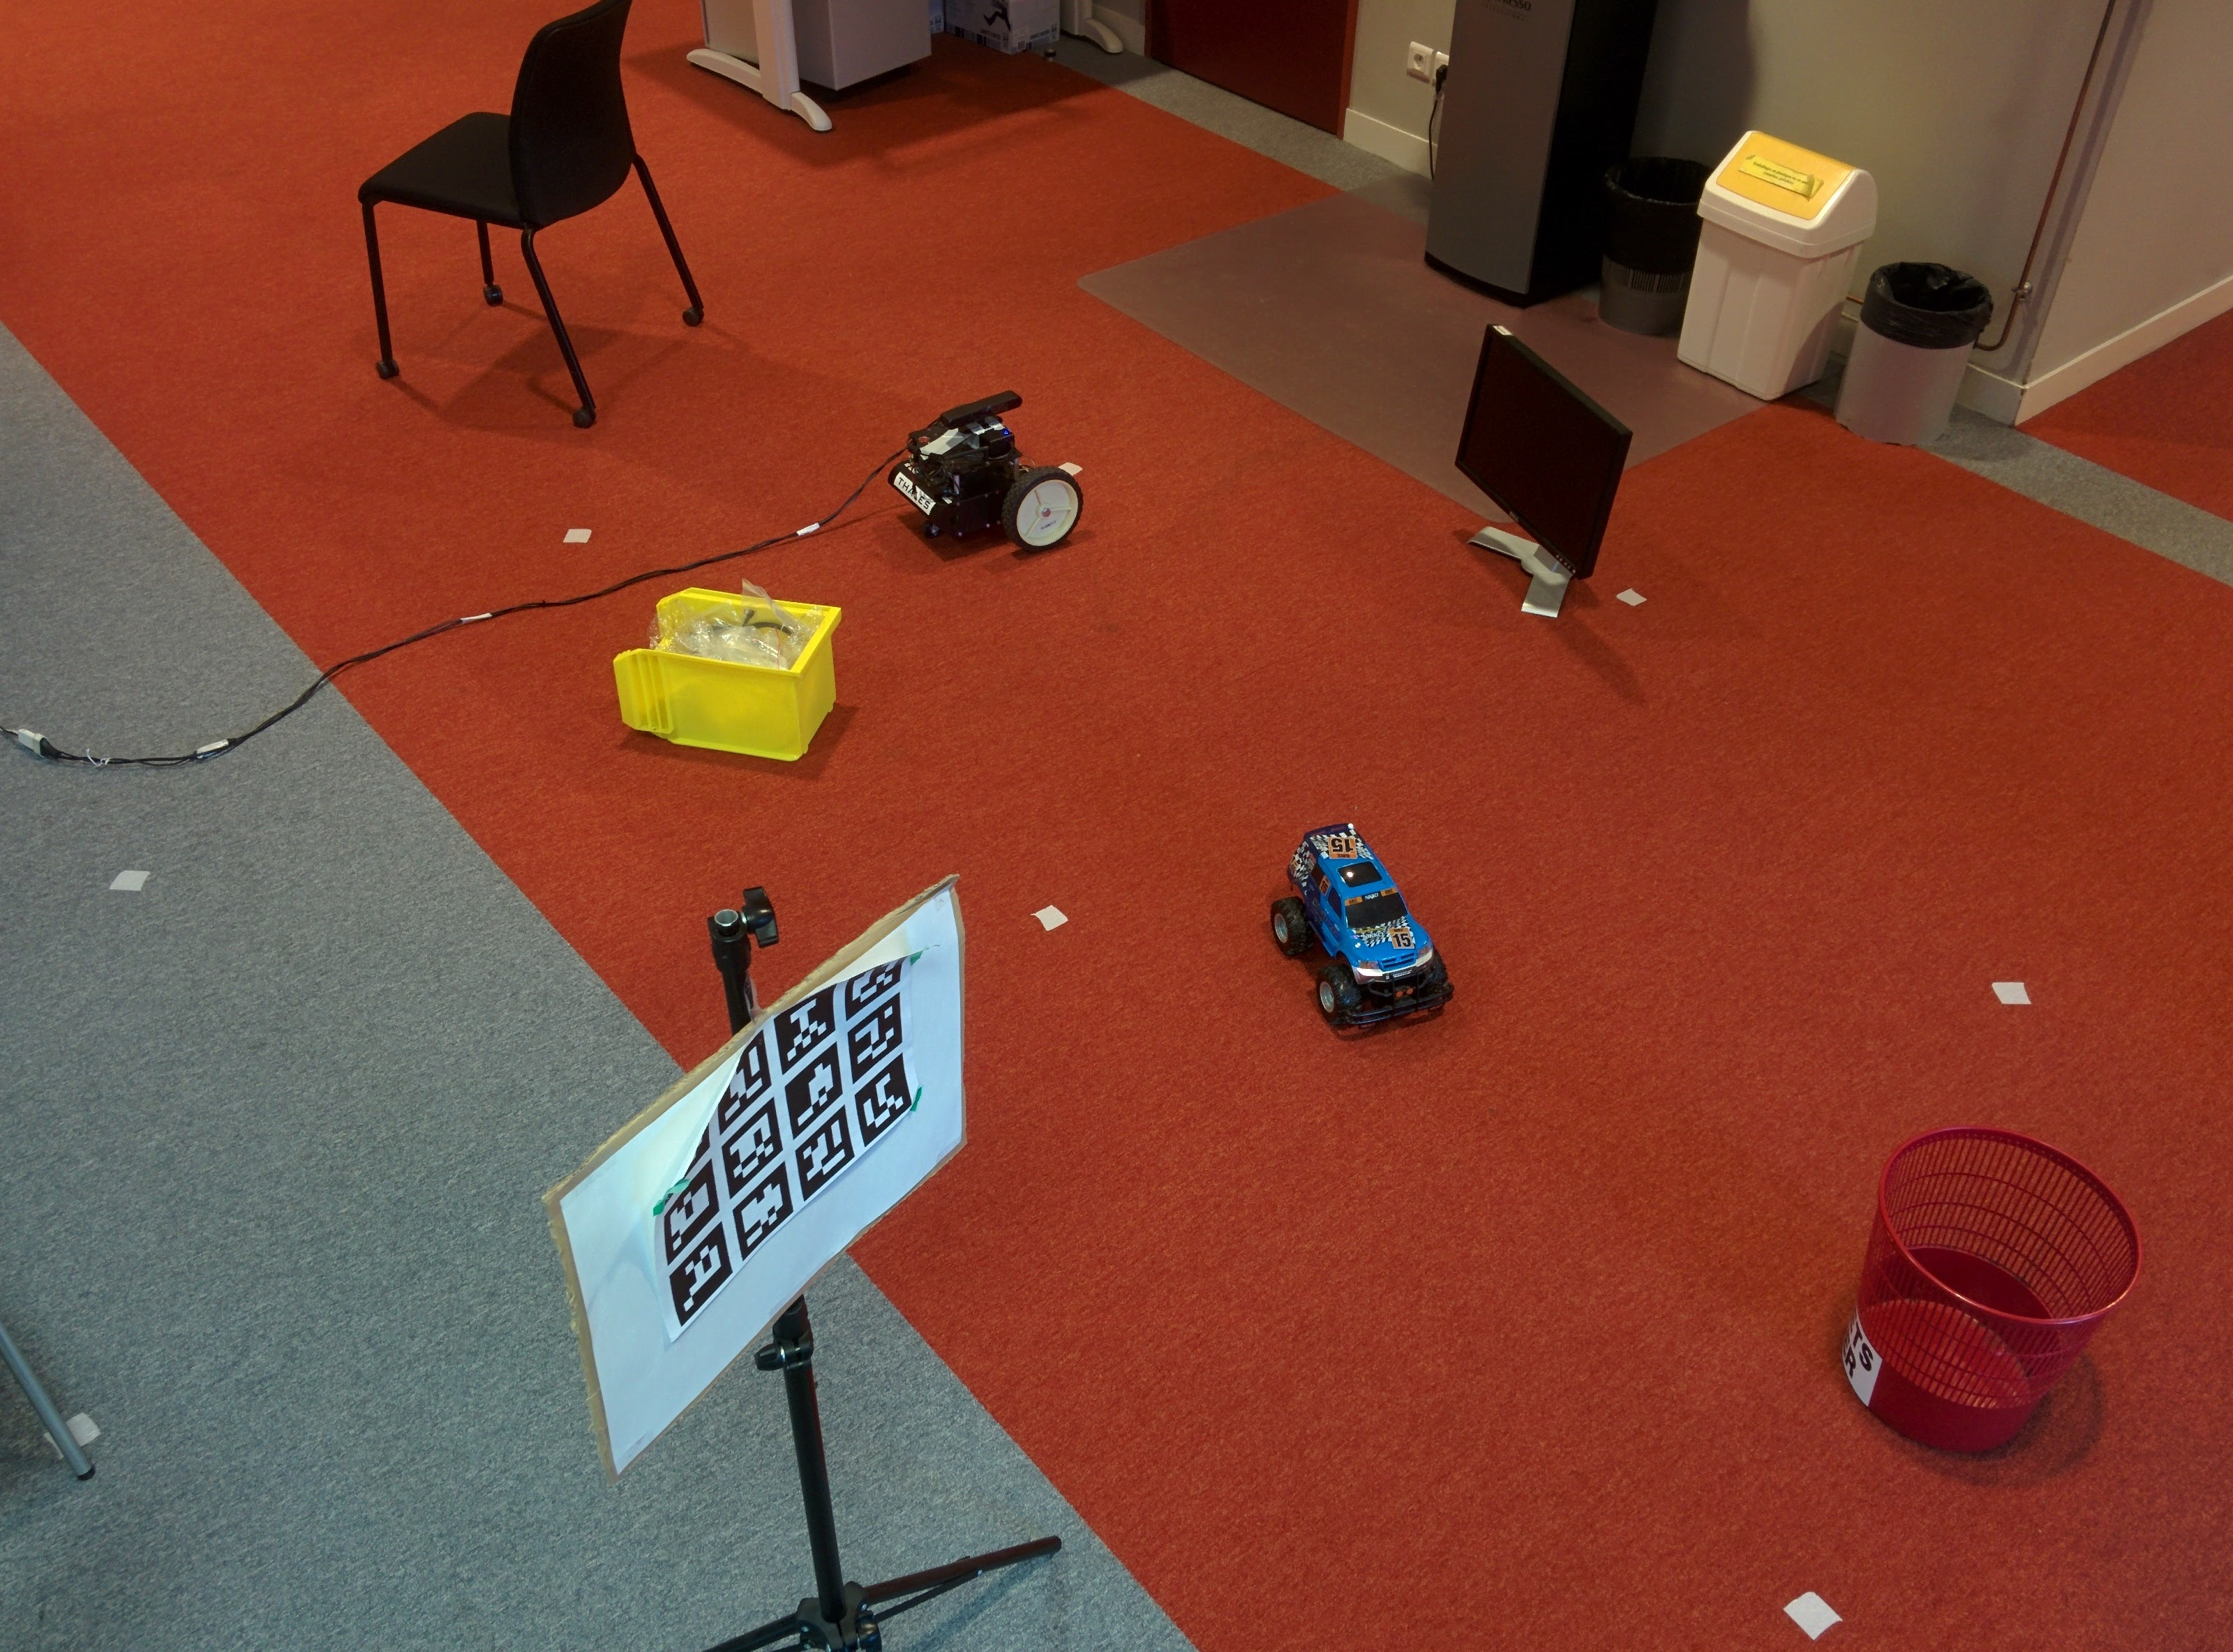
\includegraphics[width=0.8\textwidth]{exp2.jpg}\end{center}
	\label{fig:exp2}
	\caption{Un des placement des objets choisi pour le deuxième expriment}
\end{figure}

\begin{figure}[H]
	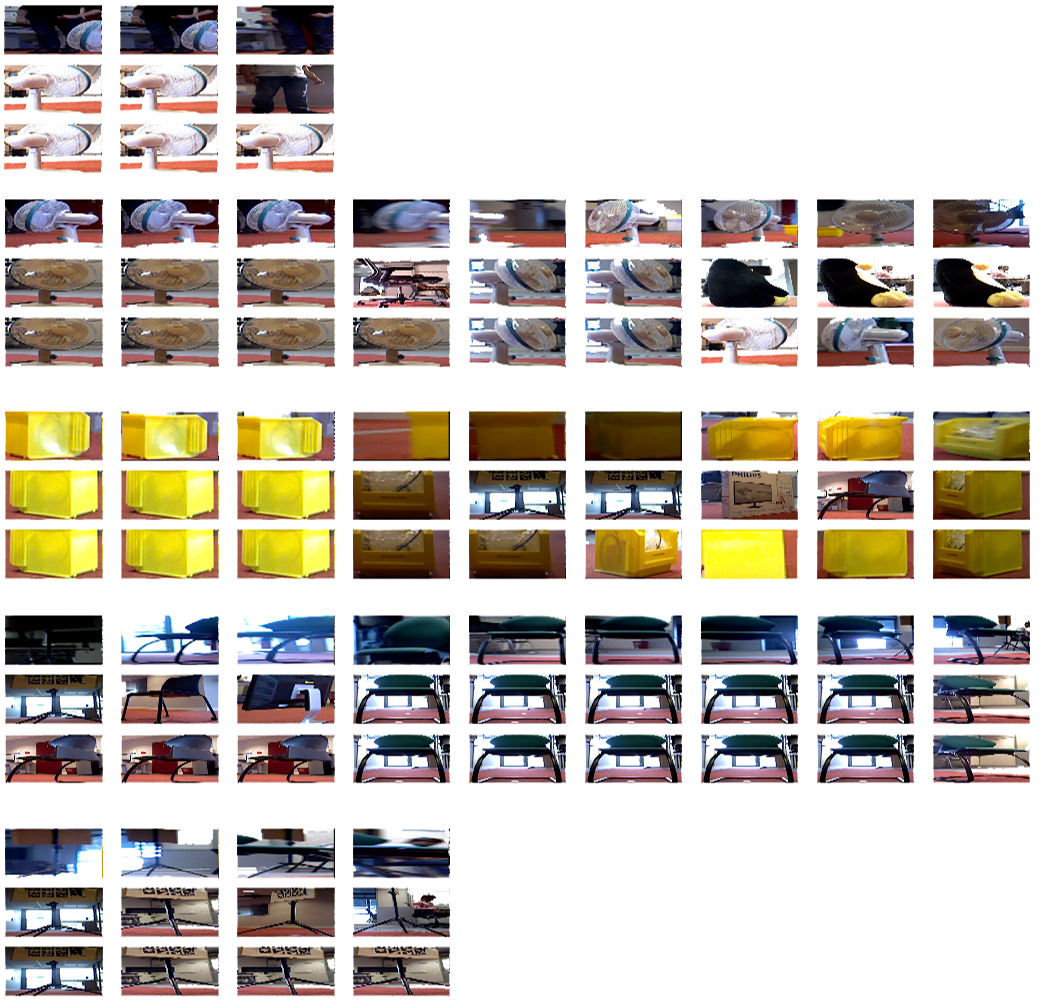
\includegraphics[width=\textwidth]{multi_recon2.png}
	\label{fig:recon}
	\caption{\textbf{Reconnaissance Multi-cible} - Quatre entre les cinq objets présentes dans la scène ont été reconnus bien reconnu avec une estimation d'orientation raisonnable. Le première objet (personne) était mal segmenté ensemble avec le ventilateur. }
\end{figure}

Les résultat de l'expriment montre que le système est capable de gérer ce cas beaucoup plus complexe, pourtant avec une réduction des taux de reconnaissance. Quelques améliorations proposés dans la section suivante pourrait être utiles pour une meilleur sa performance. Un exemple de la reconnaissance multi-cible est mis dans les annexes.  
